\cotefile{1}
\scanpage{92}

Indeed, $\overset{\inserted{30}}{27}$ is a special case of theorem 2, and ($\overset{\inserted{31}}{28}$) follows from it by passage to the limit as $n\to+\infty$. \inserted{\textcolor{red!75!black}{$*$}} \deleted{In particular, taking $f(\unsure{r|s})=\unsure{r|s}^{\unsure{p|r}}$, $\unsure{p|r}>0$, one obtains} \inserted{For another special case of corollary 1,} let $p,q,\deleted{\unsure{r}}s$ be such that

\reversemarginpar
\margin{\inserted{Let us take in particular $f(s)\equiv1$, one then obtains
\(\begingroup
\setbox0=\hbox{$\displaystyle\sum\rho_i(uv)\leq\sum\rho_i(u)\rho_i(v)$}
\textcircled{32}\quad\smash{\rlap{\begin{tikzpicture}[x=\wd0,y=1ex,baseline=0pt]
\draw[red!75!black,line width=.8pt] (-.02,2.2)--(1.04,1.9);
\draw[red!75!black,line width=.8pt] (-.025,1.8)--(-.04,-1.7)--(1.05,-2.0)--(1.04,1.9);
\end{tikzpicture}}}\box0\endgroup\)\unsure{:|.}
Taking into account \deleted{(21)} \inserted{number 1, theorem 3}, for $p=1$, \deleted{and \unsure{let}} \inserted{one concludes from this} that if the second side is finite, then $uv$ is a Fredholm operator. \deleted{As a \unsure{consequence}} Now if \deleted{\unsure{$\sum\lambda_i$}} \inserted{$E=G$}, one has
\deleted{whence $|\mathrm{Tr}(uv)|\leq\sum|\lambda_i(uv)|\leq\sum\rho_i(uv)$}
$|\mathrm{Tr}\,uv|\leq\deleted{\unsure{\sum\rho_i(v)|\sum}}\inserted{\sum\rho_i(uv)}$
\deleted{(\unsure{fundamental} \unsure{inequality} (21), for $p=1$) whence $|\mathrm{Tr}\,uv|\leq\sum\rho_i(u)\rho_i(v)$. As a \unsure{result} \unsure{one has}}
\deleted{(number 2, \unsure{theorem})} \inserted{(number 1, theorem \unsure{3|2})}.
\uline{Corollary 2}. Let $E,F$ be two Hilbert spaces, $u$ a \unsure{compact|compact} linear map from $E$ to $F$, $v$ a \unsure{compact|compact} linear map from $F$ to $G$, suppose $\sum\rho_i(u)\rho_i(v)<+\infty$, then $vu$ is a Fredholm operator, and one has
\(\begingroup
\setbox0=\hbox{$\displaystyle\begin{array}{ll}(33)&|\mathrm{Tr}\,uv|\leq\sum\rho_i(u)\rho_i(v)\\&\deleted{\illegible{3}}\end{array}$}
\smash{\rlap{\begin{tikzpicture}[x=\wd0,y=1ex,baseline=0pt]
\draw[red!75!black,line width=1pt] (0.03,3.2)--(1.06,3.15) (0,3.0)--(-0.02,-2.8)--(1.01,-2.7)--(1.03,2.8);
\draw[black,line width=.55pt] (0.02,3.3)--(1.05,3.0)--(1.04,-2.85)--(-0.01,-3.0);
\draw[black,line width=.55pt] (.40,.8)..controls(.58,1.25)and(.87,.7)..(.98,.25)--(1.01,-2.2);
\draw[black,line width=.6pt] (.39,-.8)--(.36,-2.4)--(.45,-.7)--(.44,-2.35)--(.52,-.6)--(.51,-2.3)--(.60,-.7)--(.59,-2.3)--(.68,-.9)--(.67,-2.3)--(.76,-1.0)--(.75,-2.35)--(.84,-1.1)--(.83,-2.3)--(.91,-1.0)--(.90,-2.3)--(.99,-1.2)--(.98,-2.3);
\end{tikzpicture}}}\box0\endgroup\).
\unsure{This|Corollary} \unsure{statement specifies|gives again the fact} that the product of two H.-S. operators is a Fredholm operator \deleted{\unsure{is}}. Generalize the inequality of (29).}}
\normalmarginpar

\[
\begin{array}{ll}
\deleted{\unsure{\sum}}\quad(34)&\displaystyle\frac1p+\frac1q=\frac1s\qquad(p,q,s\geq0)
\end{array}
\]

put $f(\unsure{\rho|s})=s^s$, \deleted{one has \unsure{therefore} \illegible{1} \unsure{corollary 1 gives}} the inequality \deleted{of the \unsure{corollary}} (\unsure{31|34}) gives

\[
\left(\sum_{i=1}^{n}\rho_i(uv)^s\right)^{1/s}\leq\left(\sum_{i=1}^{n}(\rho_i(u)\rho_i(v))^s\right)^{1/s}
\]

Now the Hölder inequality \deleted{\unsure{says} \unsure{$\sum$}, \unsure{that the conjugate exponents}} \inserted{\deleted{\unsure{be well known}}}
\deleted{$\sum(\rho_i(u))^s(\rho_i(v))^s\leq$}
\inserted{the second side is} bounded above by $\left(\sum\rho_i(u)^p\right)^{1/p}\left(\sum\rho_i(v)^q\right)^{1/q}$. Consequently:

\reversemarginpar
\margin{
\begin{tikzpicture}[x=1em,y=1em,baseline=0pt]\draw[red!75!black,line width=.8pt] (.15,0)..controls(.14,-.25)and(.10,-.48)..(.12,-.65);
\draw[red!75!black,line width=.65pt] (.22,.03)--(.19,-.70);
\draw[blue!35!black,line width=.35pt] (.18,.01)--(.15,-.67);
\draw[black,line width=.6pt] (0,-1.35)..controls(.08,-2.3)and(.16,-3.8)..(.20,-4.75)..controls(.18,-4.90)and(.18,-4.94)..(.13,-4.94);
\draw[black,line width=.5pt] (.19,-4.80)--(.26,-5.55);\end{tikzpicture}}
\normalmarginpar
\uline{Corollary 2}. (``\uline{Operator Hölder inequality \deleted{for}}'').\smash{\rlap{
\begin{tikzpicture}[x=1em,y=1ex,baseline=0pt]\draw[red!75!black,line width=.8pt] (-8.4,-.75)..controls(-7.4,-1.0)and(-6.6,-.96)..(-6.1,-.75)..controls(-5.5,-.68)and(-4.8,-.8)..(-4.5,-.75)..controls(-3.3,-.82)and(-1.5,-1.05)..(-.6,-.85);\end{tikzpicture}}}
\inserted{\deleted{\unsure{$u$}}} \deleted{\unsure{If $u$ is}}
Let $E,F,G$ be three Hilbert spaces, let $u$ be a compact operator from $E$ to $F$, $v$ a compact operator from $F$ to $G$, then one has, for every \deleted{\unsure{integer} $\geq1$} $(p,q,s)$ \deleted{\unsure{and every} $p$} satisfying (34), and every integer $n>1$

\[
\begin{array}{ll}(35)&\displaystyle
\left(\sum_{i=1}^{n}\rho_i(uv)^r\right)^{\unsure{1/r|1/s}}\leq
\left(\sum_1^n\rho_i(u)^p\right)^{1/p}\left(\sum_1^n\rho_i(v)^q\right)^{1/q}
\end{array}
\]

\deleted{In particular}

\[
\begin{array}{ll}(36)&\displaystyle\deleted{\left(\sum_i\rho_i(uv)^s\right)^{1/s}\leq
\left(\sum_i\rho_i(u)^p\right)^{1/p}\left(\sum_i\rho_i(v)^q\right)^{1/q}}
\end{array}
\]

\reversemarginpar
\margin{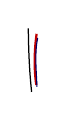
\begin{tikzpicture}[x=1em,y=1em,baseline=0pt]\draw[black,line width=.45pt] (.04,.2)..controls(.05,-.65)and(.08,-1.35)..(.16,-2.1);
\draw[red!75!black,line width=.8pt] (.34,0)..controls(.27,-.5)and(.23,-1.2)..(.33,-1.85);
\draw[blue!40!black,line width=.4pt] (.38,-.15)..controls(.25,-.7)and(.35,-1.55)..(.35,-1.92);\end{tikzpicture}}
\normalmarginpar
\[
\begingroup
\setbox0=\hbox{$\displaystyle\begin{array}{l}
\deleted{\unsure{\mathcal N_r(uv)|N_r(uv)}\leq\mathcal N_p(u)\mathcal N_q(v)}\\[.6ex]
\inserted{\|uv\|_r\leq\|u\|_p\|v\|_q}\quad\left(\frac1r=\frac1p+\frac1q\right)
\end{array}$}
\smash{\rlap{
\begin{tikzpicture}[x=\wd0,y=1ex,baseline=0pt]\draw[red!75!black,line width=1pt] (-.04,4.0)..controls(.18,3.8)and(.47,4.35)..(.72,4.3);
\draw[red!75!black,line width=1pt] (-.02,3.8)--(-.035,-3.2)..controls(.20,-3.4)and(.57,-2.9)..(1.05,-3.3);
\draw[red!75!black,line width=1.1pt] (1.02,2.5)..controls(1.05,1.4)and(1.02,-1.5)..(1.02,-3.2);
\draw[black,line width=.65pt] (.06,1.7)--(.045,.35)--(.20,3.25)--(.17,1.5)--(.30,3.8)--(.21,.1)--(.42,2.7)--(.36,.3)--(.50,2.35)--(.42,-.2)--(.58,1.25);
\draw[black,line width=.45pt] (-.04,-3.35)..controls(.27,-3.6)and(.66,-2.85)..(.96,-3.8);\end{tikzpicture}}}\box0
\endgroup
\]

\deleted{(\unsure{the sum} \illegible{3} \unsure{if all the} \illegible{1})}

The most important case of the inequality (37) is that where $s=1$, i.e. where $p$ and $q$ are two ``conjugate exponents''; \deleted{\unsure{We shall return to this} \illegible{1}} \inserted{in this case, (32) is moreover contained in} the \deleted{\unsure{inequality of the|inequalities in the} following number, in a more striking formula.}

\[
\begingroup
\setbox0=\hbox{$\displaystyle\|uv\|_1\leq\|u\|_p\|v\|_{p'}\quad\left(\frac1p+\frac1{p'}=1\right)$}
\begin{array}{ll}\textcircled{38}&\smash{\rlap{\begin{tikzpicture}[x=\wd0,y=1ex,baseline=0pt]\draw[red!75!black,line width=1pt] (.025,1.9)..controls(.27,2.3)and(.39,4.2)..(1.04,4.05);
\draw[red!75!black,line width=1pt] (-.025,1.75)--(-.05,-1.8)..controls(.25,-1.65)and(.58,.2)..(1.04,-.4);\end{tikzpicture}}}\box0\end{array}
\endgroup
\]

\deleted{(29) \unsure{which is|if all} : the \unsure{ordinary} Hölder inequality}. \inserted{(38) moreover also follows from (32), thanks to the ordinary Hölder inequality}
\par\noindent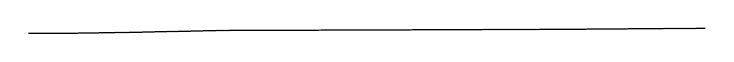
\begin{tikzpicture}[x=1cm,y=1ex,baseline=0pt]\draw[line width=.45pt] (0,0)..controls(.9,-.02)and(1.7,.15)..(2.6,.25)..controls(4.7,.28)and(6.6,.31)..(8.6,.42);\end{tikzpicture}

\reversemarginpar
\margin{\begin{tikzpicture}[x=1em,y=1em,baseline=0pt]\draw[line width=.5pt] (0,0)--(.5,.6);\end{tikzpicture}\par
Explain \unsure{the iteration|the introduction} of a \illegible{1}\par
\begin{tikzpicture}[x=1em,y=1em,baseline=0pt]\draw[line width=.55pt] (0,-.2)..controls(.65,.5)and(1.05,1.9)..(1.85,3.1);\end{tikzpicture}}
\normalmarginpar

\uline{Corollary 4}. Let $E,F,G$ be three Hilbert spaces of the same finite dimension $n$, $u$ a compact operator from $E$ to $F$, $v$ a compact operator from $F$ to $G$, $f$ \inserted{$\unsure{(t_1,-t_n)|(s_1,-s_n)}$} a \deleted{\unsure{symmetric}} function of $n$ arguments $t_i>0$ such that $f(e^{t_{\unsure{i|1}}},-e^{t_n})$ is a convex function of $(t_i)\in R^n$. Under these conditions, \inserted{if \deleted{\unsure{one of these}} \inserted{$u$ and $v$} are invertible \unsure{or|one has}} \deleted{the \unsure{formula}} \inserted{if $f$ is defined and continuous for $s_i\geq0$, one has}

\reversemarginpar
\margin{\textcolor{red!75!black}{\unsure{?}}\quad
\begin{tikzpicture}[x=1em,y=1em,baseline=0pt]\draw[red!75!black,line width=1.0pt] (0,.7)--(.12,-1.0);\end{tikzpicture}}
\normalmarginpar

\[
\begin{array}{ll}(39)&\displaystyle f(\rho_1(uv),-\rho_n(uv))\leq f(\rho_1(u)\rho_1(v),-\rho_{\unsure{n}}(u)
\end{array}
\]

Indeed, \deleted{\unsure{one knows from the}} \inserted{using the conditions} of theorem 1, 2\textsuperscript{o}, hypothesis b),

\reversemarginpar
\margin{\uline{small} \uline{type}}
\normalmarginpar

by virtue of

\[
\begin{array}{ll}(40)&\displaystyle\prod\rho_i(uv)=\deleted{f(uv)}\prod\rho_i(u)\rho_i(v)\end{array}
\]

\deleted{Indeed,} \inserted{To verify (40),} one \deleted{\unsure{squares}} \inserted{may suppose} \deleted{is reduced} that $E=F=G$, then the two sides of (35) are respectively $|\det(uv)|$ and $|\det u|\,|\det v|$ (formula (\unsure{26|16})) whence the result. If $u$ and $v$ are arbi\unsure{trary} but $f$ defined and continuous for $t_i\geq0$, (39) will still be valid by extension by continuity from the preceding case.

Give connections on the composition of operators as multiplication

\reversemarginpar\margin{93}\normalmarginpar
